\chapter{Werkstoffprüfung}
\label{sec:grundlagen}

\section{Non-Destructive Testing auf Deutsch Werkstoffprüfung}
\label{sec:ndt}
\begin{figure}[htb]
  \centering  
  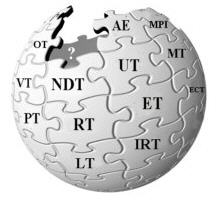
\includegraphics[scale=0.9]{img/ndtazWiki.jpg}
  \caption{NDT}
  \label{fig:ndtazWiki}
\end{figure}

Die Werkstoffprüfung umfasst verschiedene Prüfverfahren, mit denen das Verhalten und die
Werkstoffkenngrößen von normierten Werkstoffproben (Materialanalytik) oder fertigen Bauteilen
(Bauteilprüfung) unter mechanischen, thermischen oder chemischen Beanspruchungen ermittelt
werden.
Ein Werkstoff wird dabei hinsichtlich seiner Reinheit, Fehlerfreiheit oder Belastbarkeit überprüft. Nach
der Art werden die gängigen Prüfverfahren in zwei Hauptbereiche aufgeteilt: zerstörende und
zerstörungsfreie Werkstoffprüfung. Die auf die Abschätzung der Lebensdauer von Produkten und
Werkstoffen gerichteten Prüfungen fallen in das Gebiet der Umweltsimulation.\\
\\
VT:= Vor jeder anderen Zerstörungsfreien Prüfung wird eine Sichtprüfung durchgeführt. Dadurch
können erste Oberflächenfehler schnell und kostengünstig erkannt werden. Zur genaueren Analyse
ist meistens ein weiteres Prüfverfahren nötig.\\
\\
MT:= Das Magnetpulverprüfverfahren dient dem Nachweis von Fehlern wie Rissen an der Oberfläche
oder im oberflächennahen Bereich von ferromagnetischen Werkstoffen. Durch das Verfahren wird
der, an einer fehlerhaften Stelle der Oberfläche, austretende magnetische Streufluss eines geeignet
magnetisierten Werkstücks sichtbar gemacht.\\
\\
\\
PT:= Die (Farb-) Eindringprüfung ermöglicht mit einfachen Hilfsmitteln das Auffinden von Fehlern, die
bis zur Oberfläche hin offen sind. Das Verfahren kann bei jedem möglichen Material angewendet
werden.\\
\\
UT:= Mit Hilfe der Ultraschallprüfung können flächige Fehler, wie Risse oder Bindefehler besonders
gut aufgefunden werden. Die Ultraschallprüfung wird üblicherweise im Impuls-Echoverfahren
durchgeführt.\\
\\
RT:= Die Durchstrahlungsprüfung mittels Röntgen- oder Gammastrahlen eignet sich besonders zum
Auffinden von Volumenfehlern, wie Poren oder Lunker.\\
\\
\section{RT Durchstrahlungsprüfung}
\label{subsec:ndt}
Die Durchstrahlungsprüfung ist ein bildgebendes Verfahren der zerstörungsfreien Werkstoffprüfung (ZFP) zur Darstellung von Materialunterschieden.\\
Mit Röntgen- oder Gammastrahlung aus einer geeigneten Quelle (einer Röntgenröhre, einem Elektronenbeschleuniger mit Röntgentarget oder einem gammastrahlenden Radionuklid) wird die Dichte eines Bauteils auf einem Röntgenfilm abgebildet. Dort erscheint ein Projektionsbild des Bauteils. Am Grad der Schwärzung lässt sich die unterschiedliche Materialdicke oder -dichte erkennen. Je dicker oder dichter ein Bauteil, desto weniger Strahlung kann es durchdringen und desto heller erscheint die Stelle auf dem Röntgenbild.\\
\\
\subsection{Anwendung}
Die Röntgen- und Gammadurchstrahlung ist eine zerstörungsfreie Werkstoffprüfung zur Fehleraufdeckung im Inneren von Bauteilen, insbesondere an Schweißnähten von Blechen, Rohren und Behältern. Zur Prüfung sicherheitsrelevanter Bauteile bspw. von Schweißnähten (DIN EN ISO 10675-1) sowie sicherheitsrelevanter Gussteile (DIN EN 12681:2003-06 und DIN EN ISO 5579:2014-04) z. B. in Kraftwerken ist sie ein Standardverfahren.\\
Die häufigsten Fehler sind Lunker, Poren, Seigerungen und Risse. Damit diese gut erkennbar sind, müssen Strahlungsintensität, Wellenlänge der Strahlen, Dicke des Bauteils und Belichtungszeit aufeinander abgestimmt sein. Die Durchstrahlungsprüfung (Kürzel RT gem. DIN EN ISO 9712) ist geeignet zum Nachweis volumenhafter Fehler. Durch Unterschiede der Dichte zwischen Fehlstelle und Grundmaterial ist der Fehler nachweisbar. Auch feine Risse lassen sich bei geeignetem Einstrahlwinkel finden. Kontrast und Auflösung beeinflussen das Erkennen solcher Details. Der Kontrast ist abhängig von der Werkstoffdicke, der Dichte, dem Material, der Strahlerqualität/Energieintensität sowie dem Auflösungsvermögen und dem Typus des Films.\\
Zur Beurteilung der Bildgüte werden Karten (DIN EN ISO 19232-1:2013-12) mit sieben Drahtstegen unterschiedlicher Breite auf das belichtete Bauteil gelegt; die Drahtdurchmesser sind um 1,25 mm abgestuft. Anhand des dünnsten noch zu erkennenden Drahtes kann auf die kleinste erkennbare Fehlergröße geschlossen werden.\\
\\
\subsection{Eigenschaften}
Röntgen- und Gammastrahlen sind elektromagnetische Wellen. Physikalisch gleichen sie dem Licht, haben aber wesentlich kleinere Wellenlängen und dadurch höhere Frequenzen. Auf den kleinen Wellenlängen beruht die Fähigkeit, zwischen den Atomen der Materie einzudringen und mit genügend hoher Energie (Frequenz) auch durchzudringen (Bedingung: Wellenlänge muss kleiner als der Abstand zwischen den Atomen im Kristallgitter sein). Beim Durchdringen werden sie dann verschieden stark durch Fehler abgeschwächt und dadurch zeigt die austretende Strahlung Intensitätsunterschiede. Sie durchdringen Stahl bis etwa 300 mm, Leichtmetall bis 400 mm und Kupfer bis 50 mm. Das Durchdringungsvermögen der Röntgen- und Gammastrahlen ist umso höher, je kleiner die Dichte des Bauteils, die Wellenlänge der Strahlen und je größer die Frequenz ist. Gammastrahlen haben i. A. größere Eindringtiefen, weil sie kurzwelliger sind.\\
\\
\subsection{Erzeugung der Strahlen}
Gammastrahlen: Die wichtigsten Gammastrahler für die Werkstoffprüfung sind natürliche (Radium, Radon, Mesothor) und künstliche (Cobalt, Tantal, Cäsium, Thulium). Die Strahlenquelle ist ein zylinderförmiges und etwa 0,5 – 6 mm großes Präparat, das das jeweilige Radionuklid enthält. Da Gammastrahler nicht „ausgeschaltet“ werden können, sind sie gasdicht in der Strahlerkapsel mit Wolfram-Abschirmung (innen) und Blei- oder Uran-Abschirmung (außen) eingeschlossen, damit die Strahlung nicht allseitig austreten kann. Da die Strahlenquelle wesentlich kleiner als eine Röntgenröhre ist, lässt sie sich dichter an den Prüfling heranbringen, wie z. B. der Isotopenmolch, ein Gerät, das zur Schweißnahtprüfung auf Baustellen durch Rohre gezogen wird.
\\
\subsection{Fehler Nachweismöglichkeiten mit RT}

\subsubsection{Filmaufnahmen}
Die aus dem Werkstoff austretenden Strahlen treffen auf eine doppelbeschichtete Filmfolie, die auf der Rückseite mit Bleifolien abgedeckt ist, um Streustrahlen fernzuhalten. Intensitätsunterschiede setzen sich in Schwärzungsunterschiede des Films um. Durch unterschiedlich starke Schwärzungen des Films sieht man die geometrische Form sowie die Lage des Fehlers. Die Filmaufnahme ist mit Röntgen- und Gammastrahlen möglich.
Anwendung: Kontrolle von Schweißnähten und Gussteilen mit Dicken bis zu 100 mm (Stahl) und 400 mm (Al); Revisionsuntersuchungen in Kessel-, Brücken- und Flugzeugbau.\\
\subsubsection{Durchleuchtung mit Leuchtschirm}
Röntgenstrahlen regen bestimmte Kristalle zur Abgabe sichtbarer grün-gelber Strahlen an. Eine mit diesen Kristallen beschichtete Platte bildet den Leuchtschirm. Auf diesem erscheint ein Schattenbild des Prüflings, jedoch mit geringer Lichtstärke. Fehler mit geringer Dichte sind auf dem Schattenbild heller, Fehler mit höherer Dichte dunkler. Der Beobachter muss durch Bleiglas vor der Streustrahlung geschützt werden.
Anwendung: Die Durchleuchtung mit Röntgenstrahlen ist für Stahldicken bis zu 20 mm, für Leichtmetalle und Kunststoffe anwendbar.\\
\subsubsection{Röntgenbild-Verstärkerröhre}
Mit Hilfe von Elektronik kann das Röntgen-Leuchtschirmbild verkleinert und verstärkt werden. Das verstärkte (hellere) Bild kann fernsehtechnisch übertragen werden, so dass der Beobachter in einem strahlengeschützten Raum sitzen kann.
Anwendung: Prüfung von Längs- und spiralgeschweißten Rohren.\\
\subsection{Art der durchdringenden Strahlung}
\begin{figure}[htb]
  \centering  
  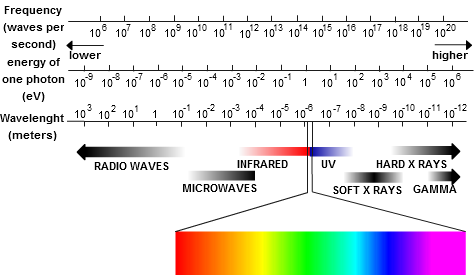
\includegraphics[scale=0.7]{img/ElectromagSpec.png}
  \caption{ElectromagSpec}
  \label{fig:ElectromagSpec}
\end{figure}
Onisierende Strahlung ist ein äußerst wichtiges Instrument der zerstörungsfreien Prüfung,es kann jedoch eine Gefahr für die menschliche Gesundheit darstellen. Aus diesem Grund sind besondere Vorsichtsmaßnahmen bei der Verwendung und dem Umgang mit ionisierender Strahlung zu beachten. Der Besitz radioaktiver Materialien und die Verwendung von Strahlung erzeugenden Geräten in den Vereinigten Staaten unterliegen strengen behördlichen Kontrollen. Die wichtigste Regulierungsbehörde für die meisten Arten und Verwendungen von radioaktiven Materialien ist die föderale Nuclear Regulatory Commission (NRC). Mehr als die Hälfte der Staaten in den USA haben jedoch eine "Vereinbarung" mit dem NRC getroffen, um die regulatorische Kontrolle der Verwendung radioaktiver Stoffe innerhalb ihrer Grenzen zu übernehmen. Im Rahmen des Einigungsprozesses müssen die Staaten Regelungen erlassen und durchsetzen, die mit denen in Titel 10 des Code of Federal Regulations vergleichbar sind. Vorschriften für die Kontrolle radioaktiven Materials in Iowa sind in Kapitel 136C des Iowa Code gefunden.\\
In den meisten Fällen werden die Arten und die Höchstmengen an radioaktivem Material, die Art und Weise, in der sie verwendet werden dürfen, und die zur Verwendung radioaktiver Stoffe berechtigten Personen in Form einer "spezifischen" Genehmigung der zuständigen Aufsichtsbehörde festgelegt. In Iowa ist diese Behörde das Iowa Department of Public Health. Bei bestimmten Instituten, die routinemäßig große Mengen zahlreicher Arten radioaktiver Stoffe verwenden, sind die genauen Mengen an Materialien und Einzelheiten der Verwendung in der Lizenz möglicherweise nicht angegeben. Stattdessen räumt die Lizenz dem Organ die Befugnis und Verantwortung ein, die spezifischen Anforderungen für die Verwendung radioaktiver Stoffe in seinen Einrichtungen festzulegen. Diese Lizenznehmer werden "Broadscope" genannt und erfordern ein Strahlensicherheits-Komitee und normalerweise einen Vollzeit-Strahlenschutzbeauftragten.

\subsection{Röntgenstrahlung}

Röntgenstrahlen sind wie jede andere Art von elektromagnetischer Strahlung. Sie können in Energiepaketen erzeugt werden, die Photonen genannt werden, genau wie Licht. Es gibt zwei verschiedene atomare Prozesse, die Röntgenphotonen erzeugen können. Einer wird Bremsstrahlung genannt und ist ein deutscher Begriff, der "bremsende Strahlung" bedeutet. Die andere wird K-Shell-Emission genannt. Sie können beide in den schweren Wolframatomen vorkommen. Wolfram ist oft das Material, das für das Target oder die Anode der Röntgenröhre gewählt wird.
Beide Arten, Röntgenstrahlen zu erzeugen, beinhalten eine Änderung des Zustands von Elektronen. Die Bremsstrahlung ist jedoch leichter zu verstehen, wenn man die klassische Idee verwendet, dass Strahlung emittiert wird, wenn sich die Geschwindigkeit des Elektronenstrahls auf das Wolfram ändert. Das negativ geladene Elektron verlangsamt sich nach dem Schwingen um den Kern eines positiv geladenen Wolframatoms. Dieser Energieverlust erzeugt Röntgenstrahlung. Elektronen werden durch den positiv geladenen Kern elastisch und inelastisch gestreut. Das inelastisch gestreute Elektron verliert Energie, die als Bremsstrahlung erscheint. Elastisch gestreute Elektronen (die rückgestreute Elektronen enthalten) werden im Allgemeinen durch größere Winkel gestreut. Bei der Wechselwirkung werden viele Photonen unterschiedlicher Wellenlängen erzeugt, aber keines der Photonen hat mehr Energie, als das Elektron hätte beginnen müssen. Nach dem Aussenden des Spektrums der Röntgenstrahlung wird das ursprüngliche Elektron abgebremst oder gestoppt.
\begin{figure}[htb]
  \centering  
  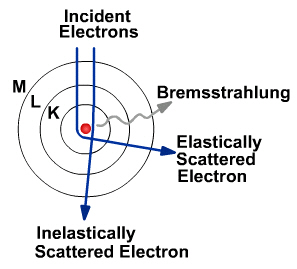
\includegraphics[scale=0.7]{img/Bremsstrahlung.jpg}
  \caption{Bremsstrahlung}
  \label{fig:Bremsstrahlung}
\end{figure}
\subsubsection{Bremsstrahlung}
Röntgenröhren erzeugen Röntgenphotonen, indem sie einen Elektronenstrom auf Energien von mehreren hundert Kilovolt mit Geschwindigkeiten von mehreren hundert Kilometern pro Stunde beschleunigen und zu einem schweren Targetmaterial kollidieren. Die abrupte Beschleunigung der geladenen Teilchen (Elektronen) erzeugt Bremsstrahlungsphotonen. Röntgenstrahlung mit einem kontinuierlichen Spektrum von Energien wird in einem Bereich von einigen keV bis zu einem Maximum der Energie des Elektronenstrahls erzeugt. Targetmaterialien für industrielle Röhren sind typischerweise Wolfram, was bedeutet, dass die Wellenfunktionen der gebundenen Wolframelektronen benötigt werden. Die inhärente Filtration einer Röntgenröhre muss berechnet werden, die durch die Menge kontrolliert wird, mit der das Elektron in die Oberfläche des Targets eindringt, und durch die Art des vorhandenen Vakuumfensters.\\
Die Bremsstrahlungsphotonen, die innerhalb des Targetmaterials erzeugt werden, werden abgeschwächt, wenn sie typischerweise 50 Mikrometer Targetmaterial passieren. Der Strahl wird durch das Aluminium- oder Beryllium-Vakuumfenster weiter gedämpft. Die Ergebnisse sind eine Eliminierung der Photonen mit niedriger Energie, 1 keV bis 15 keV, und eine signifikante Reduktion des Teils des Spektrums von 15 keV bis 50 keV. Das Spektrum von einer Röntgenröhre wird weiter durch die Filterung modifiziert, die durch die Auswahl von Filtern verursacht wird, die in dem Aufbau verwendet werden.

Das Applet unten erlaubt dem Benutzer, ein Elektron sichtbar zu machen, das mit einem schweren Zielmaterial beschleunigt und interagiert. Das Diagramm zeigt die Anzahl der Bremsstrahlungs-Photonen als Funktion der Energie. Nach einigen Ereignissen kann das "Aufbauen" des Diagramms durch Drücken der Schaltfläche "Automatisieren" erfolgen.
\subsection{Gammastrahlung}
Gammastrahlung ist eine der drei Arten natürlicher Radioaktivität. Gammastrahlen sind elektromagnetische Strahlung, wie Röntgenstrahlen. Die anderen beiden Arten natürlicher Radioaktivität sind Alpha- und Beta-Strahlung, die in Form von Teilchen vorliegen. Gammastrahlen sind die energiereichste Form elektromagnetischer Strahlung mit einer sehr kurzen Wellenlänge von weniger als einem Zehntel Nanometer.

Gammastrahlung ist das Produkt von radioaktiven Atomen. Abhängig vom Verhältnis von Neutronen zu Protonen in seinem Kern kann ein Isotop eines bestimmten Elements stabil oder instabil sein. Wenn die Bindungsenergie nicht stark genug ist, um den Kern eines Atoms zusammenzuhalten, wird das Atom als instabil bezeichnet. Atome mit instabilen Kernen verändern sich ständig infolge des Ungleichgewichts der Energie im Kern. Mit der Zeit zerfallen die Kerne von instabilen Isotopen spontan oder wandeln sich in einem Prozess, der als radioaktiver Zerfall bekannt ist. Verschiedene Arten von durchdringender Strahlung können von dem Kern und / oder seinen umgebenden Elektronen emittiert werden. Nuklide, die radioaktiv zerfallen, heißen Radionuklide. Jedes Material, das messbare Mengen eines oder mehrerer Radionuklide enthält, ist ein radioaktives Material.
Typen Strahlung, die durch radioaktives Zerfallsmaterial erzeugt wird.
Wenn ein Atom radioaktiv zerfällt, emittiert es eine oder mehrere Strahlungsformen mit ausreichender Energie, um die Atome zu ionisieren, mit denen es interagiert. Ionisierende Strahlung kann aus subatomaren Teilchen mit hoher Geschwindigkeit bestehen, die aus dem Kern ausgestoßen werden, oder aus elektromagnetischer Strahlung (Gammastrahlen), die entweder vom Kern oder den Orbitalelektronen emittiert wird.
\begin{figure}[htb]
  \centering  
  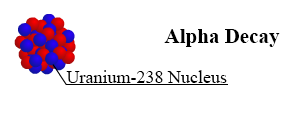
\includegraphics[scale=0.7]{img/uranium.png}
  \caption{Alpha-Zerfall}
  \label{fig:uranium}
\end{figure}

 Mit einem Uran-238-Nukleus während des Alpha-Zerfalls geschieht.
 \subsubsection{Alpha Strahlen}
 Bestimmte Radionuklide mit hoher Atommasse (Ra226, U238, Pu239) zerfallen durch die Emission von Alphateilchen. Diese Alpha-Teilchen sind fest gebundene Einheiten von zwei Neutronen und zwei Protonen (He4-Kern) und haben eine positive Ladung. Die Emission eines Alphateilchens aus dem Kern führt zu einer Abnahme von zwei Einheiten der Ordnungszahl (Z) und vier Einheiten der Massenzahl (A). Alphateilchen werden mit diskreten Energien emittiert, die charakteristisch für die jeweilige Transformation sind, aus der sie stammen. Alle Alphateilchen aus einer bestimmten Radionuklidtransformation haben identische Energien.
 \subsubsection{Beta Strahlen}
 Ein Kern mit einem instabilen Verhältnis von Neutronen zu Protonen kann durch die Emission eines Hochgeschwindigkeitselektrons, eines Betateilchens, zerfallen. Dies führt zu einer Nettoänderung von einer Einheit der Ordnungszahl (Z). Betateilchen haben eine negative Ladung, und die Betateilchen, die von einem spezifischen Radionuklid emittiert werden, liegen in einer Energie von nahe Null bis zu einem maximalen Wert, der für die bestimmte Transformation charakteristisch ist.
 \subsubsection{Gamma Strahlen}
 Ein Kern, der sich in einem angeregten Zustand befindet, kann ein oder mehrere Photonen (Pakete elektromagnetischer Strahlung) diskreter Energien emittieren. Die Emission von Gammastrahlen verändert nicht die Anzahl von Protonen oder Neutronen im Kern, sondern bewirkt stattdessen, dass der Kern von einem höheren in einen niedrigeren Energiezustand (instabil bis stabil) bewegt wird. Die Gammastrahlenemission folgt häufig dem Beta-Zerfall, dem Alpha-Zerfall und anderen Kernzerfallsprozessen.

\begin{figure}[htb]
  \centering  
  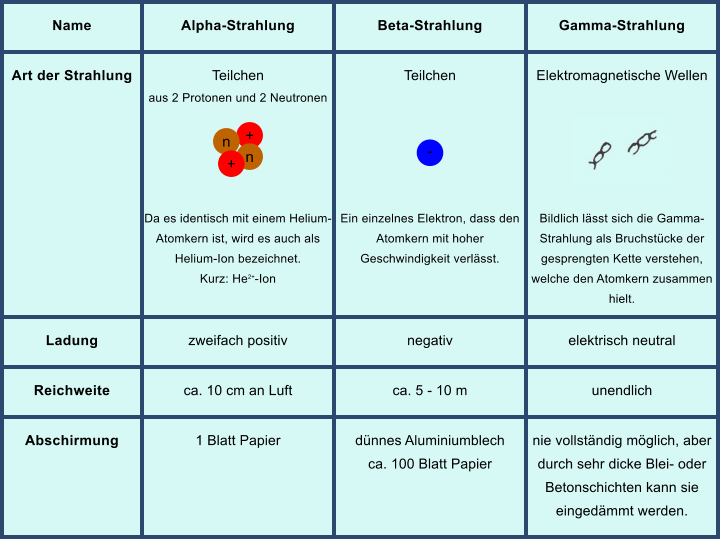
\includegraphics[scale=0.7]{img/strahlen.png}
  \caption{Die ionisierende Strahlung}
  \label{fig:strahlen}
\end{figure}
\subsection{Aktivität von Radionukliden}
Die Menge, die den Grad der Radioaktivität oder das Strahlungserzeugungspotential einer gegebenen Menge an radioaktivem Material ausdrückt, ist Aktivität.
Die Curie wurde ursprünglich als diejenige Menge von radioaktivem Material definiert, die mit der gleichen Geschwindigkeit wie ein Gramm reines Radium zerfällt.
Die Curie wurde seitdem genauer definiert als eine Menge radioaktiven Materials in
3.7 x 1010 Atome zerfallen pro Sekunde. Die Einheit des Internationalen Systems (SI) für die Aktivität ist das Becquerel (Bq), die Menge an radioaktivem Material, in der ein Atom pro Sekunde umgewandelt wird.
Die Radioaktivität einer gegebenen Menge an radioaktivem Material hängt nicht von der Masse des vorhandenen Materials ab.
Zum Beispiel könnten zwei Ein-Curie-Quellen von Cs-137 sehr unterschiedliche Massen haben, abhängig von dem relativen Anteil von nicht-radioaktiven Atomen, die in jeder Quelle vorhanden sind. Die Radioaktivität wird als die Anzahl von Curie oder Becquerel pro Massen- oder Volumeneinheit ausgedrückt.
\begin{figure}[htb]
  \centering  
  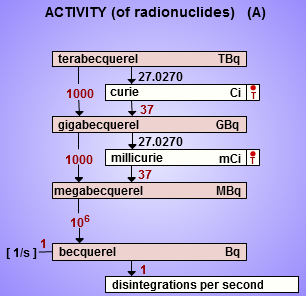
\includegraphics[scale=0.8]{img/activity.png}
  \caption{Radioaktivität}
  \label{fig:activity}
\end{figure}
Die Konzentration der Radioaktivität oder die Beziehung zwischen der Masse des radioaktiven Materials und der Aktivität wird "spezifische Aktivität" genannt. Die spezifische Aktivität wird ausgedrückt als die Anzahl der Curie oder Becquerel pro Massen- oder Volumeneinheit. Jedes Gramm Cobalt-60 enthält etwa 50 Curies. Iridium-192 enthält 350 Curies für jedes Gramm Material.
Je kürzer die Halbwertszeit, desto weniger Material wird benötigt, um eine bestimmte Aktivität zu erzeugen oder zu curieren.
Die höhere spezifische Aktivität von Iridium führt zu physikalisch kleineren Quellen. Dies ermöglicht es den Technikern, die Quelle näher an den Film zu legen, während die geometrischen Unschärfeanforderungen auf dem Röntgenbild beibehalten werden.
Diese Unschärfebedingungen können möglicherweise nicht erfüllt werden, wenn eine Quelle mit einer geringen spezifischen Aktivität bei ähnlichen Abständen von Quelle zu Film verwendet wird.
\subsection{Isotopenabfallrate (Halbwertszeit)}
Jedes Radionuklid zerfällt mit seiner eigenen einzigartigen Geschwindigkeit, die durch keine chemischen oder physikalischen Prozesse verändert werden kann. Ein nützliches Maß für diese Geschwindigkeit ist die Halbwertszeit des Radionuklids. Die Halbwertszeit ist definiert als die Zeit, die erforderlich ist, damit die Aktivität eines bestimmten Radionuklids auf die Hälfte seines Anfangswertes absinkt. Mit anderen Worten, die Hälfte der Atome ist zu einem stabileren Zustand zurückgekehrt. Die Halbwertszeiten von Radionukliden reichen von Mikrosekunden bis Milliarden von Jahren. Die Halbwertszeit von zwei weit verbreiteten industriellen Isotopen beträgt 74 Tage für Iridium-192 und 5,3 Jahre für Kobalt-60. Genauere Berechnungen können für die Halbwertszeit dieser Materialien gemacht werden, jedoch werden diese Zeiten üblicherweise verwendet.
\begin{figure}[htb]
  \centering  
  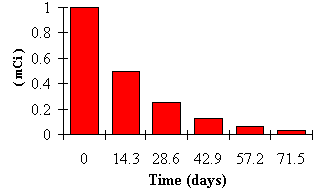
\includegraphics[scale=0.5]{img/halbwertszeit.png}
  \caption{Isotopen Halbwertszeit}
  \label{fig:halbwertszeit}
\end{figure}

Das Applet bietet eine interaktive Darstellung der radioaktiven Zerfallsreihen. Die vier dargestellten Serien sind Th232, Ir192, Co60, Ga75 und C14. Wählen Sie mit den Optionsfeldern die Serie aus, die Sie studieren möchten. Beachten Sie, dass Kohlenstoff-14 nicht in der Radiographie verwendet wird, sondern eines von vielen nützlichen radioaktiven Isotopen ist, die verwendet werden, um das Alter von Fossilien zu bestimmen. Wenn Sie mehr über Carbon-14 Dating erfahren möchten, folgen Sie diesem Link: Carbon-14 Dating.

Die Schaltfläche Sequence Info zeigt ein Diagramm an, das den Pfad der Reihe mit Ordnungszahlen auf der linken vertikalen Achse und die Anzahl der entlang der unteren Achse angezeigten Neutronen angibt. Farbige Pfeile repräsentieren Alpha- und Beta-Zerfälle. Um zur Hauptbenutzeroberfläche zurückzukehren, klicken Sie auf die Schaltfläche "Verwerfen".

Zu Beginn enthält eine ausgewählte Serie das gesamte Ausgangsmaterial und die Menge wird durch einen farbigen Balken auf einer vertikalen logarithmischen Skala dargestellt. Jede Zeile repräsentiert einen Faktor von zehn. Um die Sequenz um eine bestimmte Anzahl von Jahren vorwärts zu durchlaufen, können Sie die entsprechende Zahl in das Feld "Zeitschritt" eingeben und "Enter" drücken. Ein negativer Zeitschritt wird durch die Sequenz zurückverfolgen.

Sie können ein Schrittintervall in Jahren wählen und durch Drücken der "Enter" -Taste jeden Schritt durchlaufen. Die Schaltfläche "Animieren" automatisiert den Fortschritt der Serie. Sie können entweder einen Zeitschritt vor der Animation wählen oder ihn auf Null setzen. Wenn der Zeitschritt bei Null bleibt, wählt das System Zeitschritte, um die Anzeigequalität zu optimieren.
\subsection{Halbwertsschicht}
Die Dicke eines gegebenen Materials, bei dem 50\% der einfallenden Energie gedämpft wurden, ist als Halbwertschicht (HVL) bekannt. Die HVL wird in Entfernungseinheiten (mm oder cm) ausgedrückt. Wie der Dämpfungskoeffizient ist es abhängig von der Photonenenergie. Die Erhöhung der Durchdringungsenergie eines Photonenstroms führt zu einer Erhöhung der HVL eines Materials.

Die HVL ist umgekehrt proportional zum Dämpfungskoeffizienten. Wenn eine einfallende Energie von 1 und eine übertragene Energie von 0,5 in die auf der vorhergehenden Seite eingeführte Gleichung eingesteckt wird, kann man sehen, dass die HVL mit m multipliziert wird.
 \begin{figure}[htb]
 \centering 
  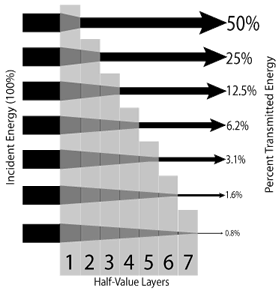
\includegraphics[scale=0.5]{img/Half-Value-Layer.png}
  \caption{Half-Value-Layer}
  \label{fig:Half-Value-Layer}
  \end{figure}


Wenn x die HVL ist, dann muss m HVL gleich 0,693 sein(da die Zahl 0,693 der Exponentenwert ist, der einen Wert von 0,5 ergibt).

\begin{figure}[htb]
  \centering  
  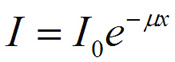
\includegraphics[scale=0.5]{img/Die_Kurve_Formel.jpg}
\end{figure}

\begin{figure}[htb]
  \centering  
  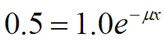
\includegraphics[scale=0.5]{img/IntensityEq5.jpg}
  \caption{IntensityEq5}
  \label{fig:IntensityEq5}
\end{figure}

  \subsubsection{Half-Value-Layer}
Die HVL wird häufig in der Radiographie verwendet, weil es einfacher ist, sich Werte zu merken und einfache Berechnungen durchzuführen. Bei einer Abschirmungsberechnung, wie sie rechts dargestellt ist, kann gesehen werden, dass, wenn die Dicke einer HVL bekannt ist, schnell bestimmt werden kann, wie viel Material benötigt wird, um die Intensität auf weniger als 1\% zu reduzieren.\\
\\
Daher sind die HVL und m wie folgt verwandt:
\begin{figure}[htb]
\centering 
  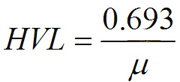
\includegraphics[scale=0.5]{img/IntensityEq6.jpg}
  \caption{IntensityEq6}
  \label{fig:IntensityEq6}
  \end{figure}
  \subsubsection{Approximate HVL für verschiedene Materialien mit Gamma Quelle}
  {\rowcolors{3}{yellow}{green}
\begin{tabular}{ |p{3cm}||p{2cm}|p{2cm}|p{2cm}|p{2cm}|p{2cm}| }
 \hline
 \multicolumn{6}{|c|}{ Half-Value Layer, mm (inch)} \\
 \hline
 Source& Concrete &Steel &Lead&Tungsten&Uranium\\
  \hline
 Iridium-192 & 44.5 (1.75)&12.7 (0.5)&4.8 (0.19)&3.3 (0.13)&2.8 (0.11)\\
  \hline
 Cobalt-60   &60.5 (2.38)&21.6 (0.85)&12.5 (0.49)&7.9 (0.31)&6.9 (0.27)\\
 \hline
\end{tabular} 
\subsubsection{Approximate HVL für verschiedene Materialien mit X-ray Quelle}

{\rowcolors{3}{yellow}{green}

\begin{tabular}{ |p{4cm}||p{3cm}|p{3cm}|  }
\hline
\multicolumn{3}{|c|}{Half-Value Layer, mm (inch)} \\
\hline
Peak Voltage (kVp) & Lead&Concrete \\
\hline
50&0.06 (0.002)& 4.32 (0.170) \\
\hline
100	&0.27 (0.010)&15.10 (0.595) \\
\hline
150	&0.30 (0.012)& 22.32 (0.879) \\
\hline
200& 0.52 (0.021) & 25.0 (0.984) \\
\hline
250& 0.88 (0.035)&28.0 (1.102)  \\
\hline
300& 1.47 (0.055) & 31.21 (1.229) \\
\hline
400& 2.5 (0.098)& 33.0 (1.299) \\
\hline
1000&7.9 (0.311) & 44.45 (1.75)\\
\hline
\end{tabular} \\


\subsection{Ionisation}
Da sich die durchdringende Strahlung in Materie von Punkt zu Punkt bewegt, verliert sie ihre Energie durch verschiedene Wechselwirkungen mit den Atomen, auf die sie trifft.
Die Geschwindigkeit, mit der dieser Energieverlust abhängt, durch welche von der Art und Energie der Strahlung und der Dichte und der atomaren Zusammensetzung der Materie tritt es passiert.
Die verschiedenen Arten von durchdringender Strahlung übertragen ihre Energie hauptsächlich durch Anregung und Ionisation von Orbitalelektronen. Der Begriff „Anregung“ wird verwendet, um eine Wechselwirkung zu beschreiben, wo Elektronen Energie von einem vorbeifahrenden geladenen Teilchen zu erwerben, sind jedoch nicht vollständig von ihrem Atom entfernt. Aufgeregte Elektronen können anschließend Energie in Form von Röntgenstrahlen während des Prozesses der Rückkehr in einen niedrigeren Energiezustand emittieren. Der Begriff "Ionisierung" bezieht sich auf die vollständige Entfernung eines Elektrons von einem Atom nach der Übertragung von Energie von einem passierenden geladenen Teilchen. Bei der Beschreibung der Intensität der Ionisation wird häufig der Begriff "spezifische Ionisation" verwendet. Dies ist definiert als die Anzahl von Ionenpaaren, die pro Weglängeneinheit für eine gegebene Art von Strahlung gebildet werden.

\begin{figure}[htb]
  \centering  
  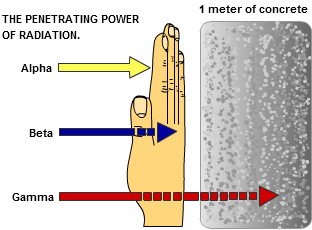
\includegraphics[scale=0.5]{img/Ionisation.png}
  \caption{Ionisation}
  \label{fig:Ionisation}
\end{figure}

Aufgrund ihrer doppelten Ladung und relativ langsamen Geschwindigkeit haben Alphateilchen eine hohe spezifische Ionisierung und eine relativ kurze Reichweite in der Materie (einige Zentimeter in Luft und nur Bruchteile von einem Millimeter im Gewebe). Betateilchen haben eine viel geringere spezifische Ionisierung als Alphateilchen und im allgemeinen einen größeren Bereich. Zum Beispiel haben die relativ energiereichen Betateilchen von P32 eine maximale Reichweite von sieben Metern in der Luft und acht Millimeter im Gewebe. Die niederenergetischen Betas von H3 werden andererseits nur von sechs Millimetern Luft oder sechs Mikrometern Gewebe gestoppt.
Gammastrahlen, Röntgenstrahlen und Neutronen werden als indirekt ionisierende Strahlung bezeichnet, da sie, ohne Ladung, nicht direkt Impulse an die Orbitalelektronen abgeben, wie es Alpha- und Betateilchen tun. Elektromagnetische Strahlung durchläuft Materie, bis eine Wechselwirkung mit einem Teilchen möglich ist. Wenn das Teilchen ein Elektron ist, kann es genug Energie erhalten, um ionisiert zu werden, woraufhin es eine weitere Ionisierung durch direkte Wechselwirkungen mit anderen Elektronen bewirkt. Als Ergebnis kann indirekt ionisierende Strahlung (z. B. Gamma, Röntgenstrahlen und Neutronen) die Freisetzung von direkt ionisierenden Teilchen (Elektronen) tief in einem Medium verursachen. Da diese neutralen Strahlungen nur zufällige Begegnungen mit Materie erfahren, haben sie keine endlichen Bereiche, sondern werden exponentiell abgeschwächt. Mit anderen Worten, ein gegebener Gammastrahl hat eine bestimmte Wahrscheinlichkeit, irgendein Medium irgendeiner Tiefe zu durchqueren.\\
Neutronen verlieren Energie in Materie durch Kollisionen, die kinetische Energie übertragen. Dieser Vorgang wird Moderation genannt und ist am effektivsten, wenn die Materie, mit der die Neutronen kollidieren, etwa die gleiche Masse wie das Neutron hat. Wenn die Neutronen einmal auf die gleiche durchschnittliche Energie abgebremst sind wie die Materie, mit der sie interagiert (thermische Energien), haben sie eine viel größere Chance, mit einem Kern in Wechselwirkung zu treten. Solche Wechselwirkungen können dazu führen, dass Material radioaktiv wird oder Strahlung abgeben kann.

\subsection{Newtons umgekehrtes quadratisches Gesetz für die Intensität}

Jede Punktquelle, die ihren Einfluss gleichmäßig in alle Richtungen ausbreitet, ohne eine Begrenzung ihrer Reichweite zu haben, wird dem Gesetz des umgekehrten Quadrats folgen. Dies ergibt sich aus streng geometrischen Überlegungen. Die Intensität des Einflusses bei jedem gegebenen Radius (r) ist die Quellenstärke dividiert durch die Fläche der Kugel. Das Gesetz des umgekehrten Quadrats, das streng geometrisch ist, gilt für verschiedene Phänomene. Punktquellen der Gravitationskraft, des elektrischen Feldes, des Lichts, des Schalls und der Strahlung folgen dem umgekehrten Quadratgesetz.
Als eines der Felder, die dem allgemeinen inversen Quadratgesetz folgen, kann eine Punktstrahlungsquelle durch das obige Diagramm charakterisiert werden, ob Sie von Röntgen, Rad oder Rem sprechen. Alle Belichtungsmaße werden durch das umgekehrte Quadratgesetz fallen.
Wenn zum Beispiel die Strahlenbelastung 100 mR / h bei 1 Inch von einer Quelle beträgt, beträgt die Belichtung 0,01 mR / h bei 100 Inch.
\begin{figure}[htb]
  \centering  
  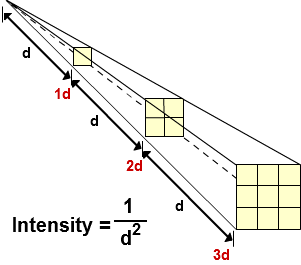
\includegraphics[scale=0.5]{img/Intensitaet.png}
  \caption{Intensität}
  \label{fig:Intensität}
\end{figure}
Das Applet unten zeigt eine radioaktive Quelle. Die Entfernung zur grünen Quelle wird unten angezeigt. Sie können auch die kleine Person und ihren Geiger-Zähler auf eine Entfernung Ihrer Wahl ziehen. Wenn die Maustaste losgelassen wird, wird ein Punkt in der Grafik gezeichnet. Die Dosierung, die die Person in der jeweiligen Entfernung erhält, wird numerisch und grafisch angezeigt. Die Grafik erlaubt es, Newtons Inverses Quadratgesetz zu bestätigen.
Wenn der Abstand zu klein ist, ist die Dosierung zu hoch und unser tapferer Techniker wird schwere medizinische Effekte haben. Um das Diagramm zu löschen, wählen Sie ein neues Material oder dasselbe aus. Bewegen Sie die Maus vom weißen Bereich zum grauen, wird der Ton ausgeschaltet!
\subsection{Wechselwirkung zwischen eindringender Strahlung
und Materie}
Wenn Röntgenstrahlen oder Gammastrahlen in ein Objekt gerichtet werden, interagieren einige der Photonen mit den Teilchen der Materie und ihre Energie kann absorbiert oder gestreut werden. Diese Absorption und Streuung wird als Dämpfung bezeichnet. Andere Photonen wandern vollständig durch das Objekt, ohne mit einem der Teilchen des Materials in Wechselwirkung zu treten. Die Anzahl der Photonen, die durch ein Material durchgelassen werden, hängt von der Dicke, Dichte und Atomzahl des Materials und der Energie der einzelnen Photonen ab.
\begin{figure}[htb]
  \centering  
  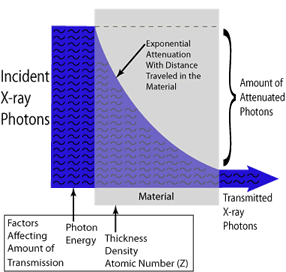
\includegraphics[scale=0.7]{img/wechselwirkungstrahlung1.png}
  \caption{wechselwirkungstrahlung1}
  \label{fig:strahlung1}
\end{figure}
Selbst wenn sie die gleiche Energie haben, bewegen sich Photonen in einem Material in unterschiedlichen Abständen, einfach aufgrund der Wahrscheinlichkeit ihrer Begegnung mit einem oder mehreren Teilchen der Materie und der Art der Begegnung.
Da die Wahrscheinlichkeit einer Begegnung mit der zurückgelegten Entfernung zunimmt, nimmt die Anzahl der Photonen, die einen bestimmten Punkt innerhalb der Materie erreichen, exponentiell mit der zurückgelegten Entfernung ab.
Wie in der Grafik rechts gezeigt, wenn 1000 Photonen auf zehn 1 cm-Schichten eines Materials gerichtet sind und eine 10\% Wahrscheinlichkeit besteht, dass ein Photon in dieser Schicht gedämpft wird, werden 100 Photonen abgeschwächt. Dies lässt 900 Fotos in die nächste Schicht, in denen 10 prosten dieser Fotos abgeschwächt werden.
Durch Fortsetzen dieses Verlaufs wird die exponentielle Form der Kurve offensichtlich.
\begin{figure}[htb]
  \centering  
  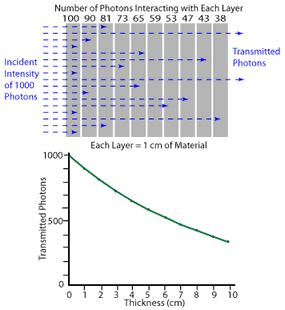
\includegraphics[scale=0.5]{img/wechselwirkungstrahlung2.png}
  \caption{wechselwirkungstrahlung2}
  \label{fig:strahlung2}
\end{figure}

Die Formel, die diese Kurve beschreibt, lautet
\begin{figure}[htb]
  \centering  
  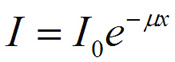
\includegraphics[scale=0.3]{img/Die_Kurve_Formel.jpg}
  \caption{DieKurveFormel}
  \label{fig:Kurve Formel}
\end{figure}














 
 
 


